%\setcounter{chapter}{7}
\chapter{Module Production for the Phase I CMS Pixel Detector Upgrade}\label{ch:phase1}

As discussed in chapter \ref{ch:lhcandcms} the CMS pixel detector will \ital{suffer} from radiation damage throughout its lifetime hence the need for periodical updates. The first version of the detector was known as phase 0, it became fully operational 2010 after solving a setback during the original starting period in 2008. In 2017 the pixel detector was replaced during the so-called phase 1 upgrade, the University of Nebraska, high energy group (UNL-HEP) played a major role in assembling and testing over 500 modules, from 2013 to 2016, which then became part of the forward region of the pixel detector (FPix). The next update of this detector (phase 2) is projected to take place in 2025 when the current detector will be reaching its limits. In this chapter we describe why the phase 0 pixel detector needed an upgrade making 

the work done by the UNL-HEP group. Some of these steps will be highlighted and described in detail as they were my contributions to this production campaign. Specially the  and highlighting 


\section{The CMS Pixel Detector Phase I Upgrade}
The CMS pixel detector is composed of two sections, the barrel section (BPix) and the forward section (FPix). Each of these sections (for phase 0) was composed of three layers originally designed to record three 3D positions (tracks) of the particles emerging from the \ital{pp} collisions. As well as to provide information to reconstruct primary and secondary vertices of decaying particles. This detector performed well during the LHC run I,{\rojo{incorporate the bunch crossing?}} taking data at the design luminosity of $1 x 10^{34} cm^{-2} s^{-1}$, which was then used in many analysis including the discovery of the Higgs bosson published in 2013. But after a few years of operation the pixel detector started to degrade due to radiation damage, causing an increase of fake rates as well as loose on resolution. Moreover, for run II the LHC planned to double the luminosity with successive increment until reach its peak of $2 x 10^{35} cm^{-2} s^{-1}$. A simulation of the performance of the pixel detector under different luminosity conditions can be seen in figure \ref{fig:red_perf}

\begin{figure}[!h]
\centering
\includegraphics[width=0.9\textwidth]{ch7/reducedperformance}
%\includegraphics[width=0.9\textwidth]{pixel/reducedperformance}
\caption[Expected performance of the original pixel detector for different luminosities.]{Expected performance of the original pixel detector under different luminosity conditions: a) track-finding efficiency; b) fake rate. Conventions are the same for both plots, considering zero pileup (blue squares), average pileup of 25 (red dots), average pileup of 50 (black diamonds), and average pileup of 100 (magenta triangles).\cite{pix_tdr}}\label{fig:red_perf}
\end{figure}

This degradation prompted the need for an improved pixel detector. It was designed to have four layers in the barrel ubicated at distances of Hena2420
and 3 layers at each endcap as shown in \ref{fig:new_pix}. better 







\begin{figure}[!h]
\centering
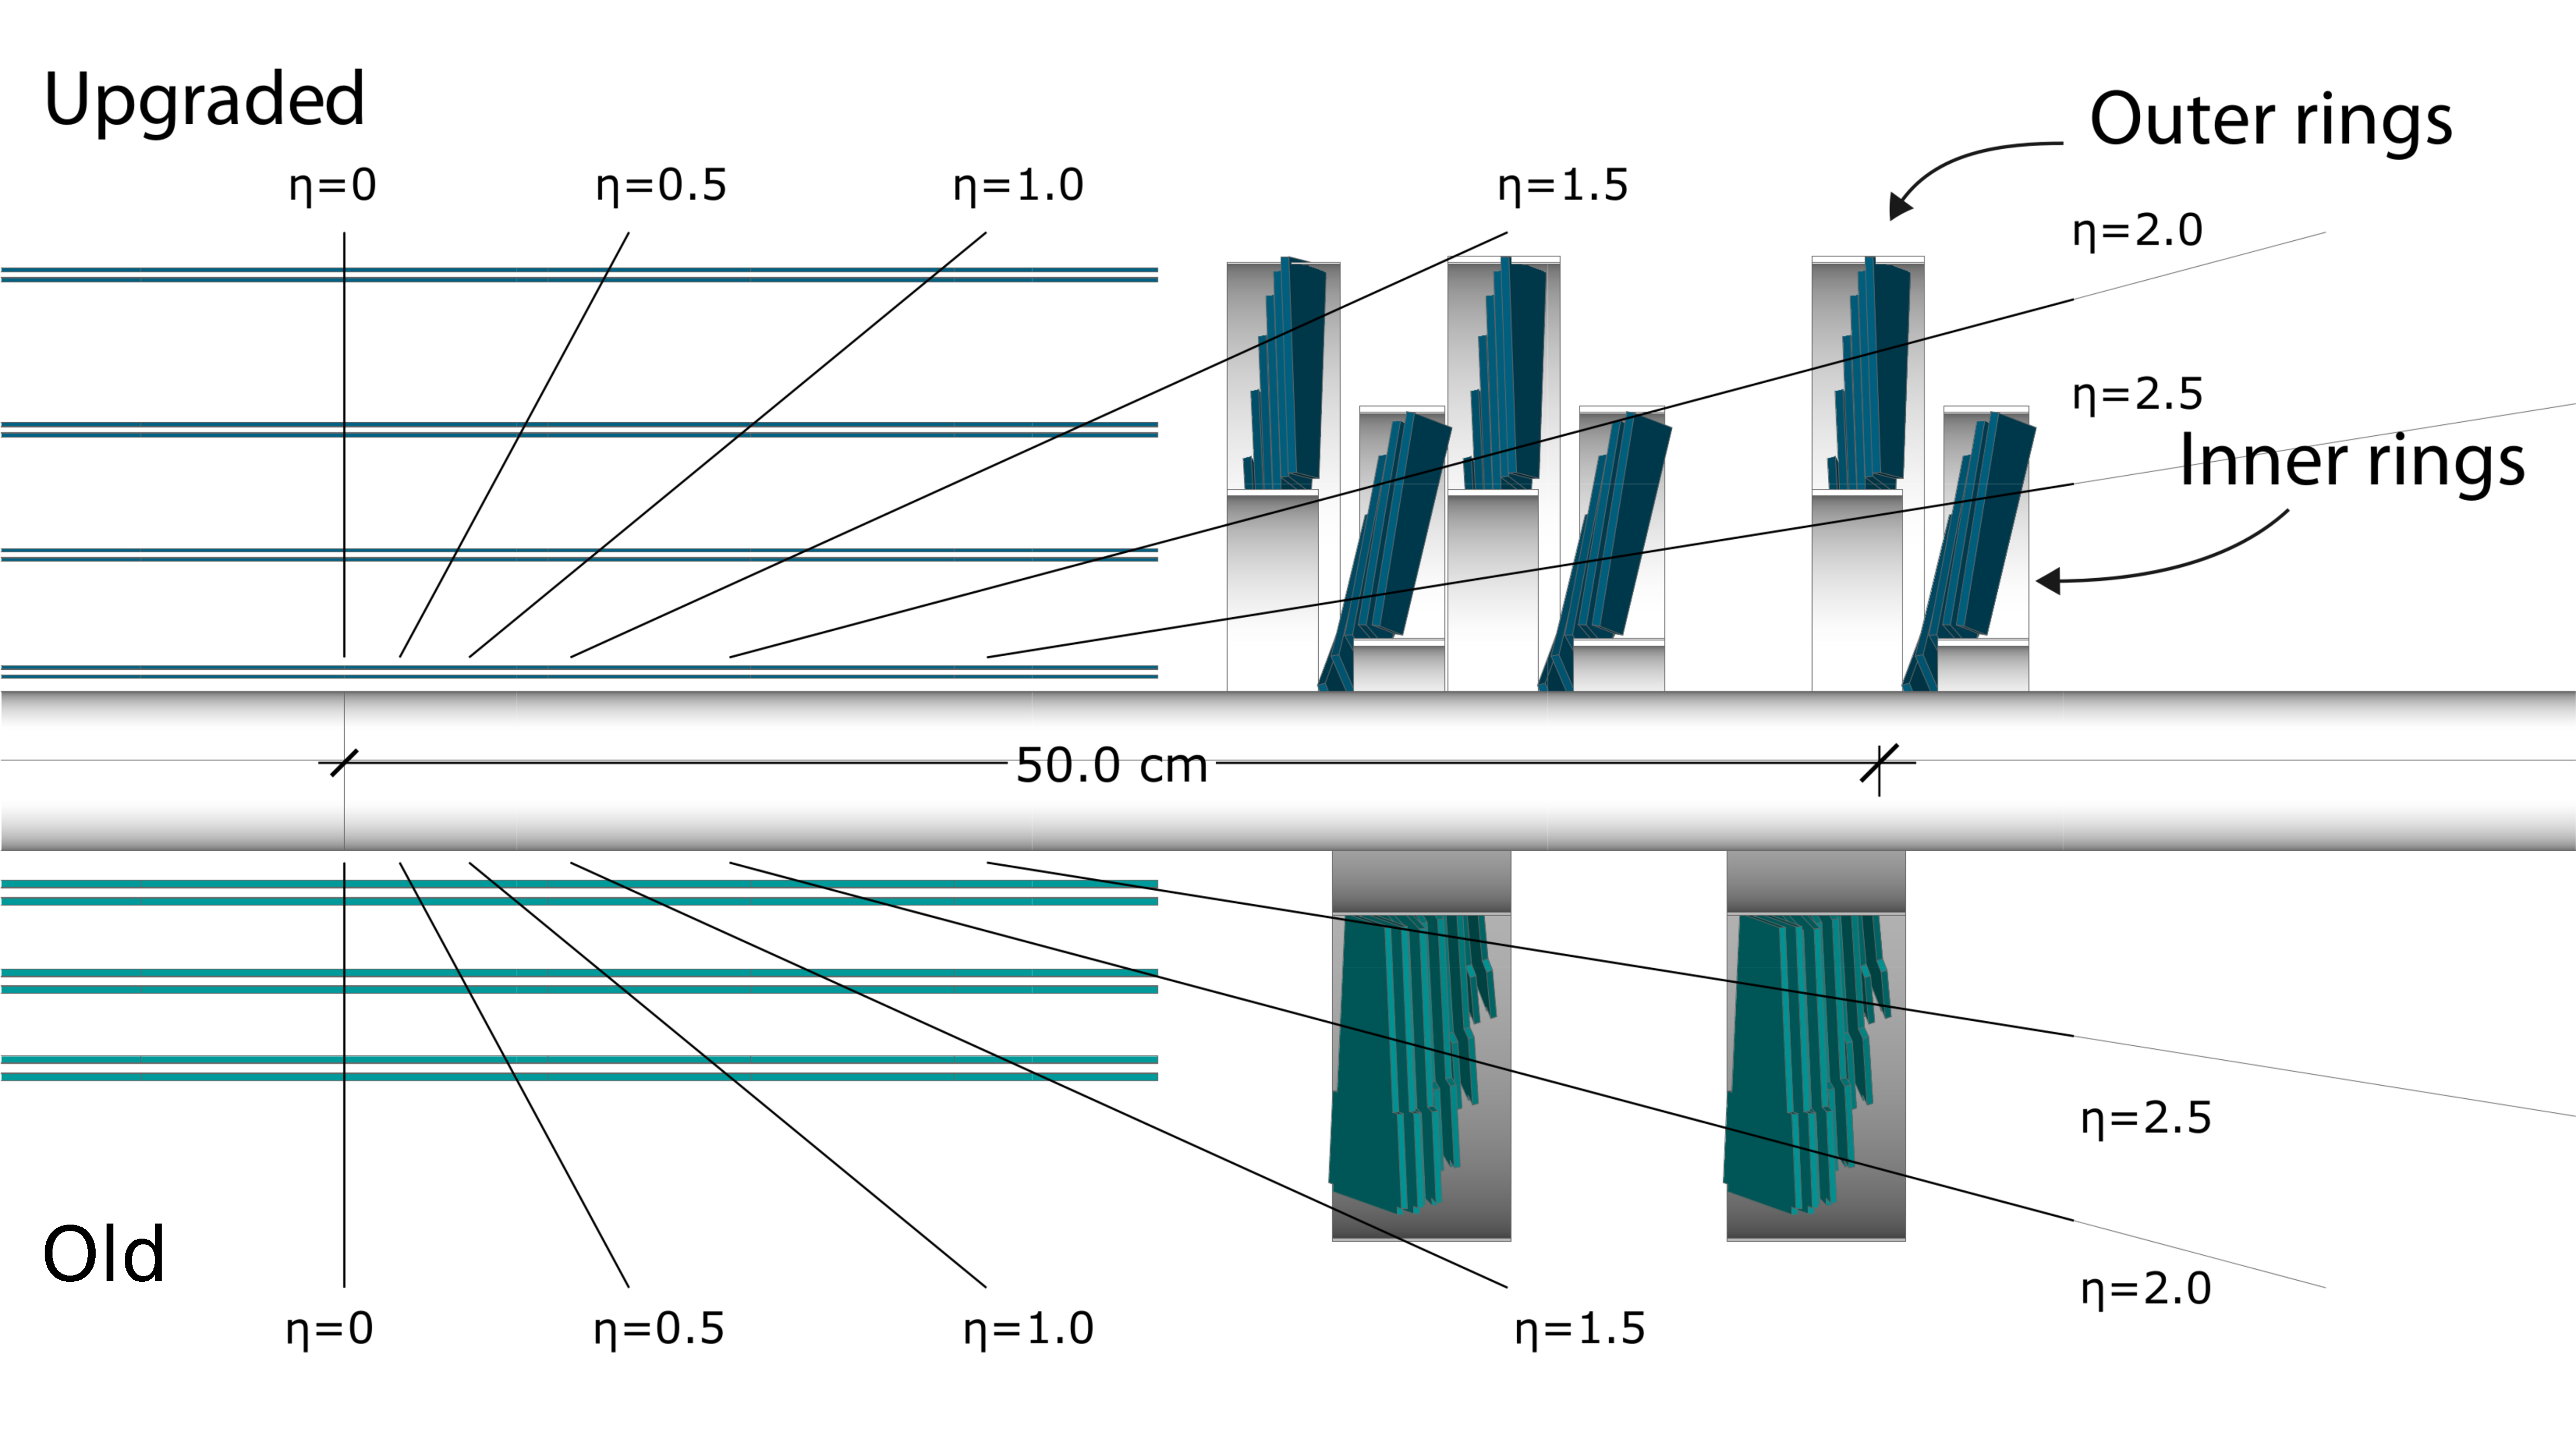
\includegraphics[width=0.6\textwidth]{../images/ch7/fpix.pdf}
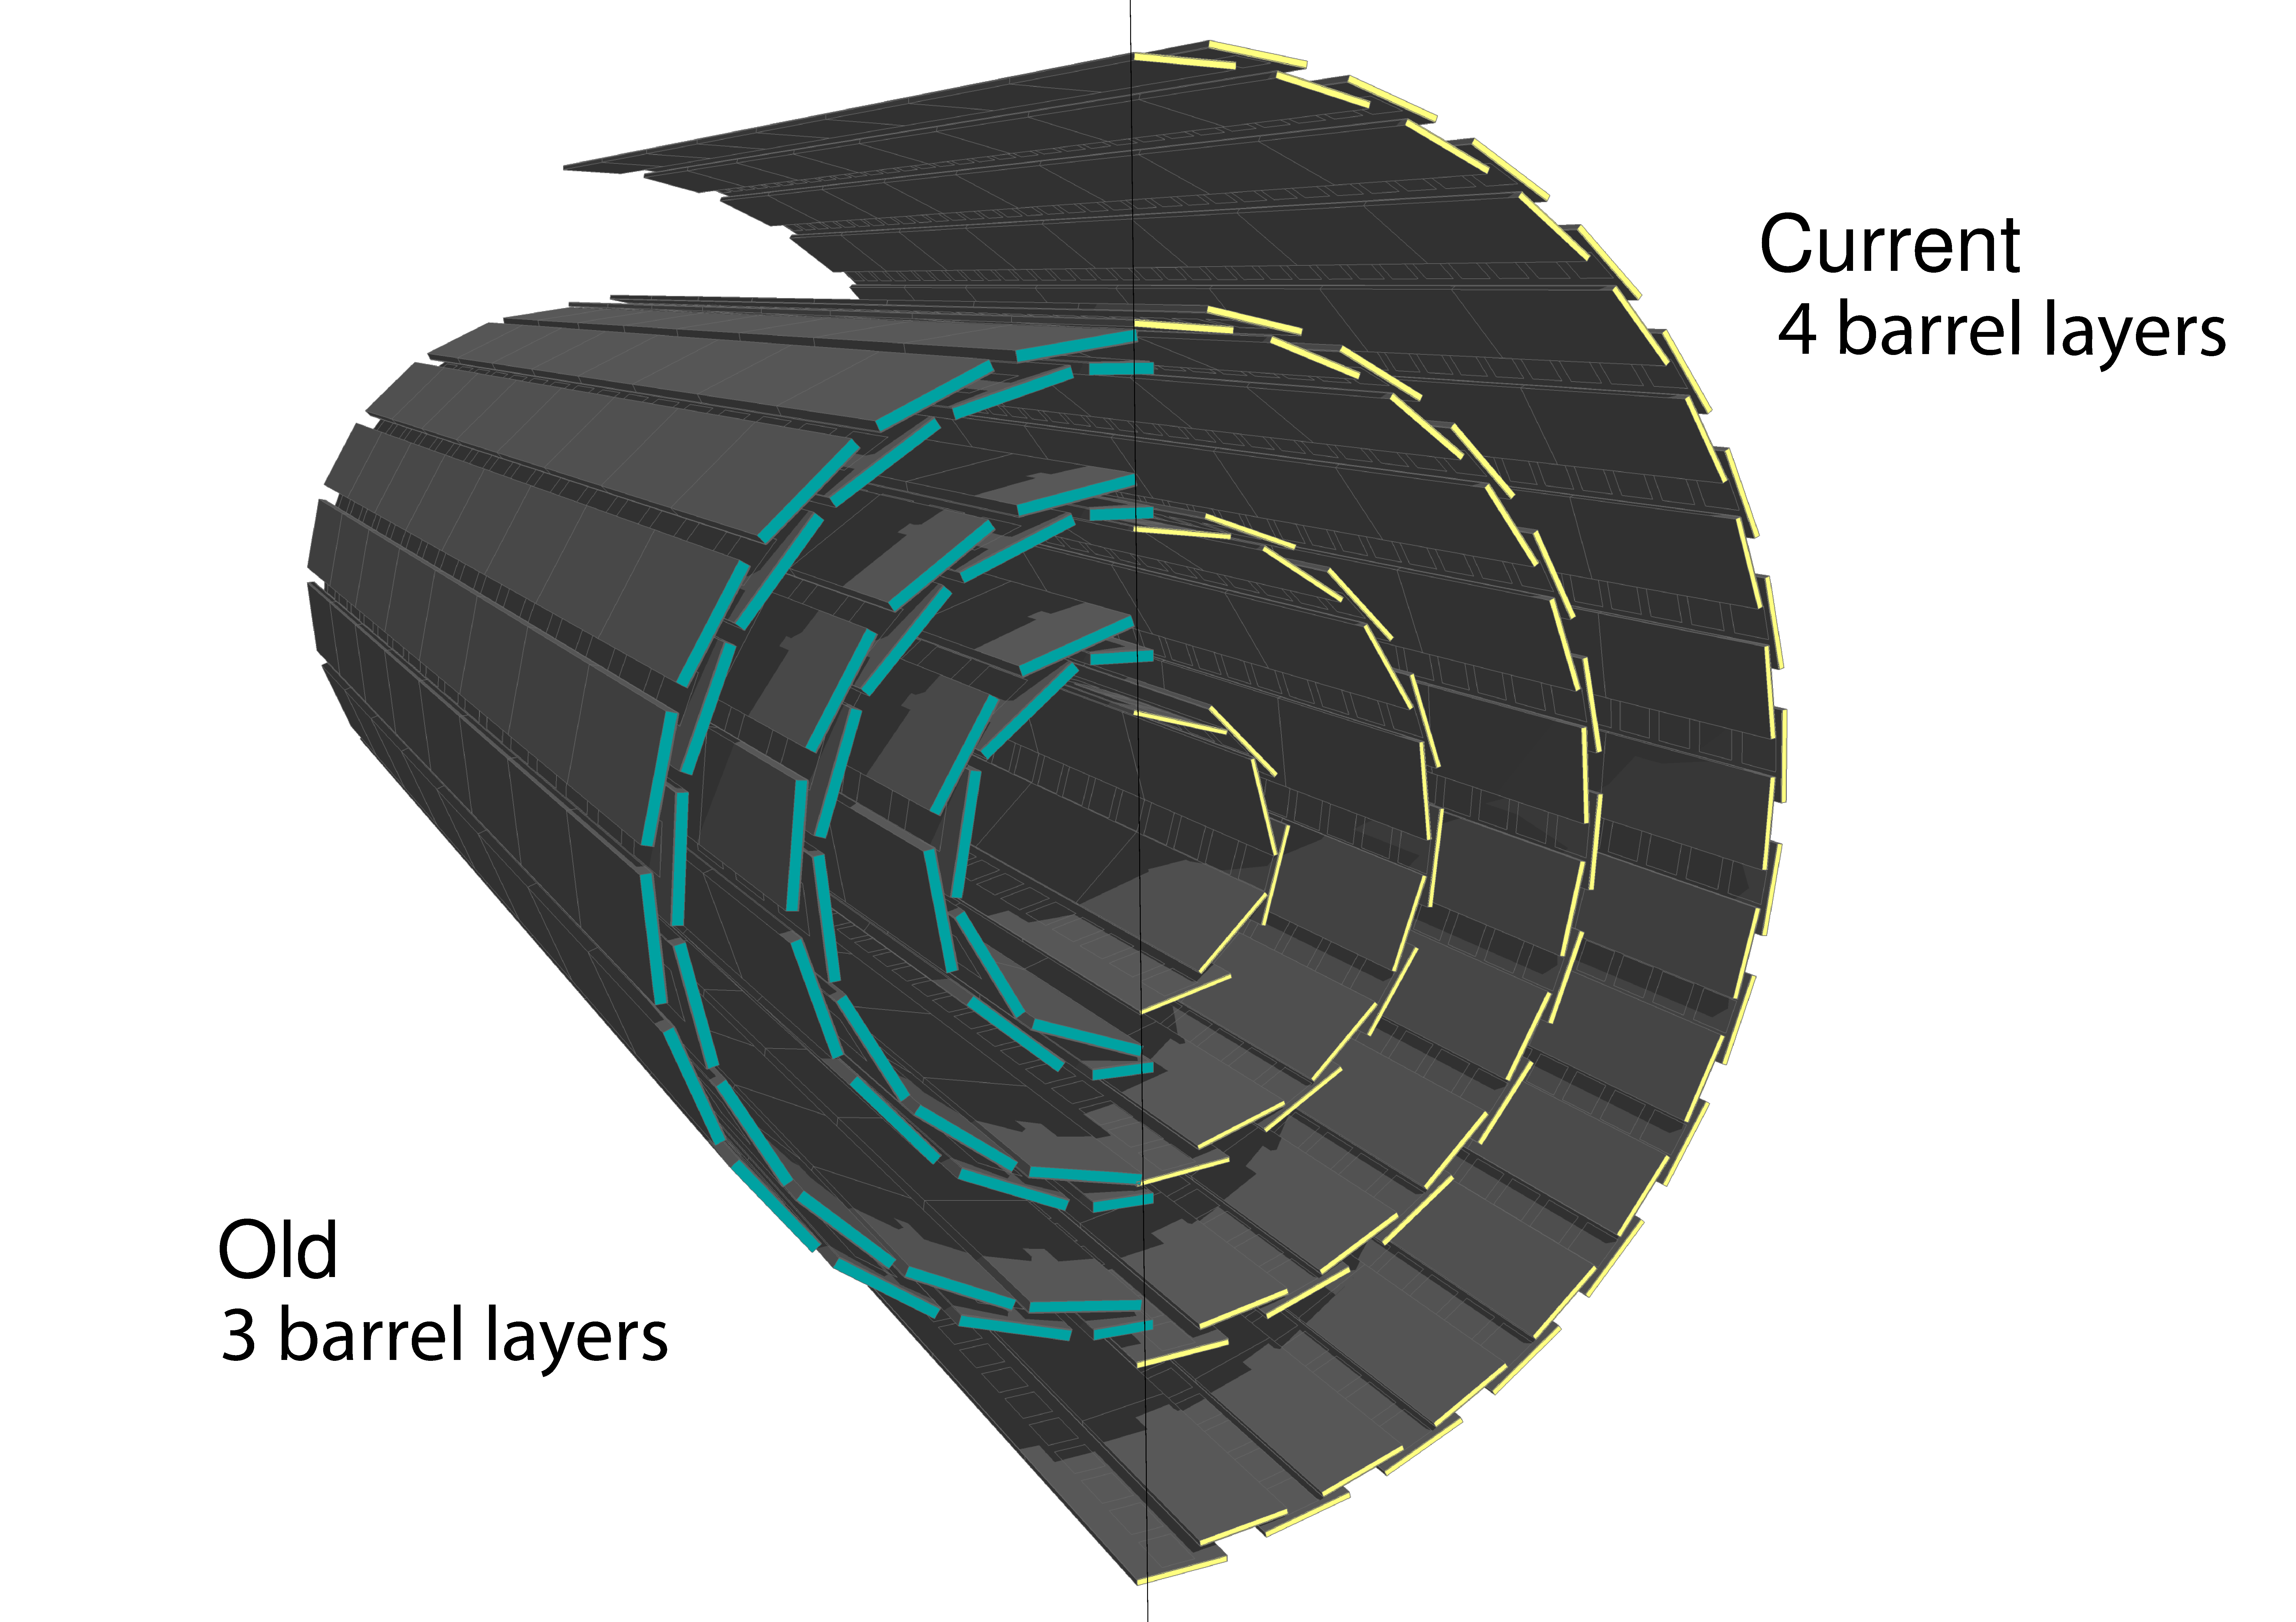
\includegraphics[width=0.39\textwidth]{../images/ch7/bpix.pdf}
\caption[Layout of the upgraded and old pixel detectors.]{Layout and comparison of the layers and disks in the upgraded (Phase I) and old (Phase 0) pixel detectors \cite{pix_tdr}.}\label{fig:new_pix}
\end{figure}

\section{Module Production at UNL}
The UNL module production workflow was designed to follow a pipeline-like as shown in figure \ref{fig:unlworkflow}

The UNL-HEP group assembly workflow started by receiving two components: a Bare Bonded Module (BBM) and a High Density Interconnect (HDI), see figure \ref{fig:bbmyhdi}. Upon receiving, a visual inspection was done on these components to assure they were in good conditions and able to enter the production chain. A image showing the sort of thing we were looking for during the visual inspection could be seen in figure \ref{fig:vis_insp}.    
 
\begin{figure}[!h]
\centering

\includegraphics[width=0.6\textwidth]{../images/ch7/gato1}

\includegraphics[width=0.39\textwidth]{../images/ch7/gato2}
\caption[Photograph of a BBM and HDI.]{Photograph of a BBM (left) and HDI (right) as were received by the UNL-HEP group.}\label{fig:bbmyhdi}
\end{figure}

\begin{figure}[!h]
  \centering
  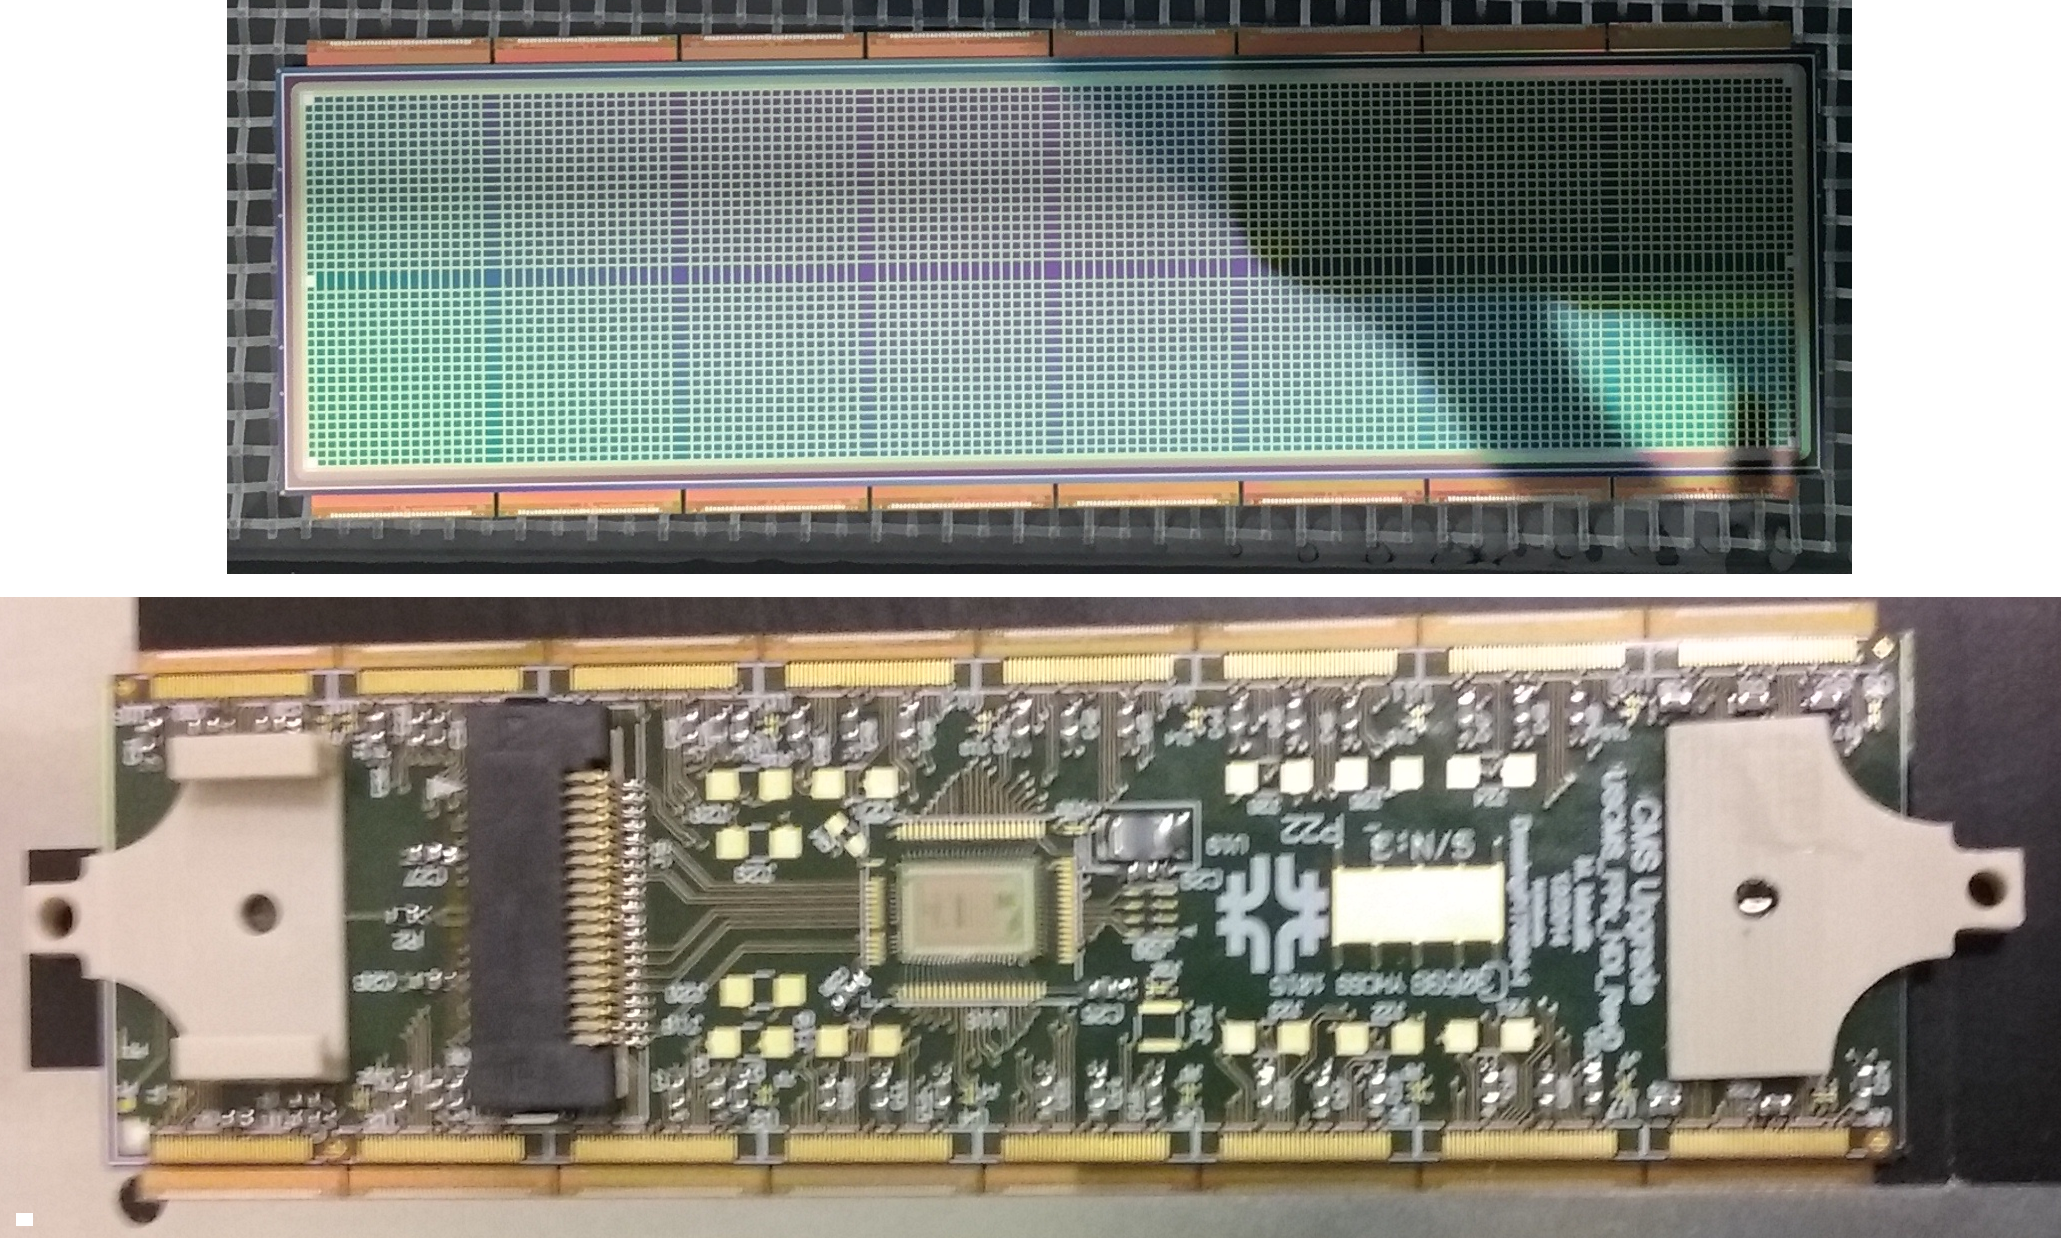
\includegraphics[width=0.7\textwidth]{../images/ch7/bbm_hdi}
  \caption[Visual inspection of a bare module.]{Visual inspection of a bare module.}\label{fig:vis_insp}
\end{figure}



\begin{figure}[!h]
  \centering
  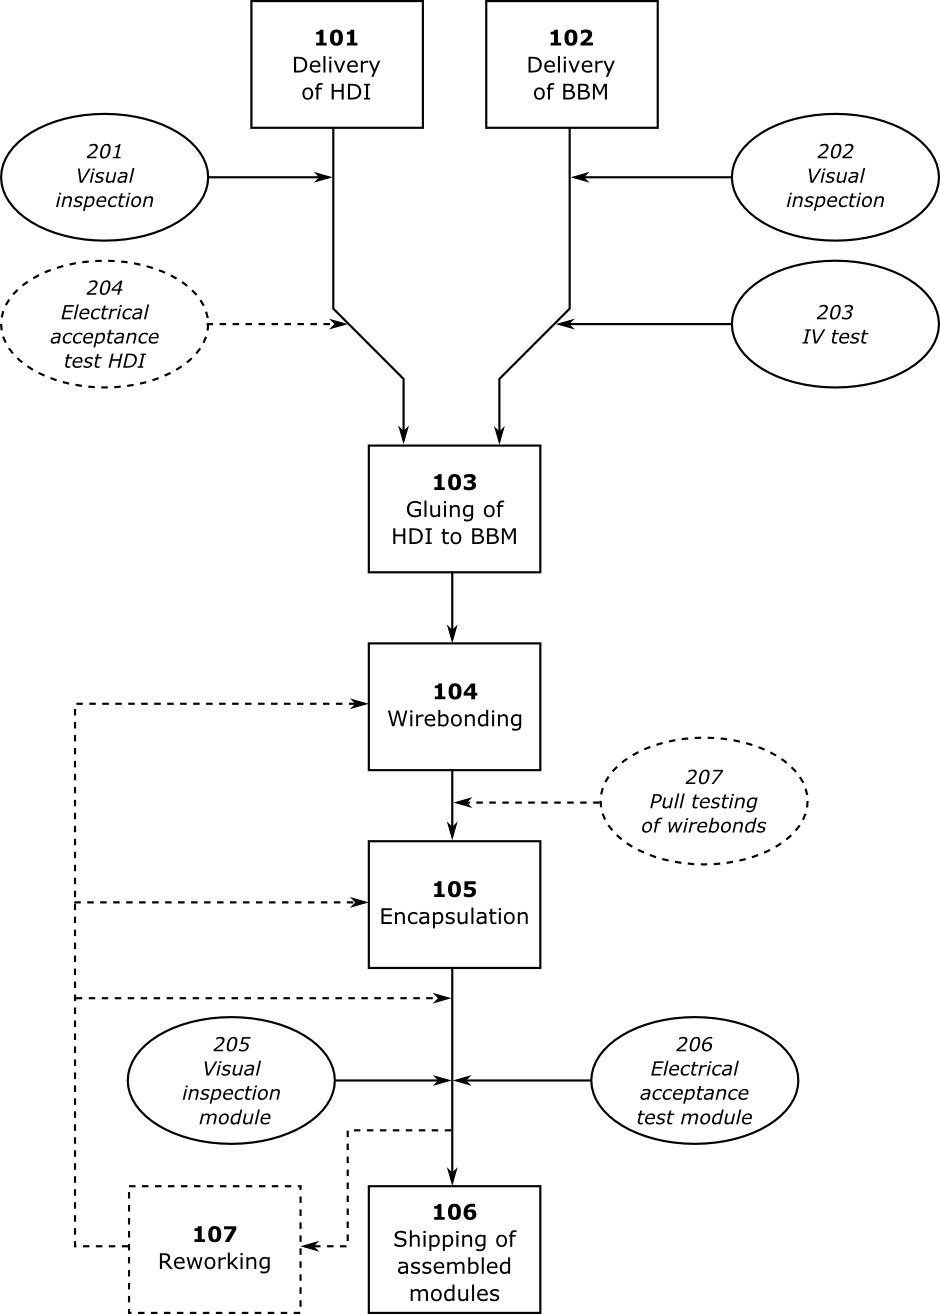
\includegraphics[width=0.7\textwidth]{../images/ch7/unl_workflow}
  \caption[UNL module assembly work flow.]{UNL module assembly work flow. Dashed lines represent occasional quality testing and reworking procedures; 10X numbers represent the stage within the assembly procedure while 20X numbers represent testing stages along the assembly procedure \cite{ph1_sop}.}\label{fig:unlworkflow}
\end{figure}


\subsection{visual inspections}



\begin{figure}[!h]
  \centering
  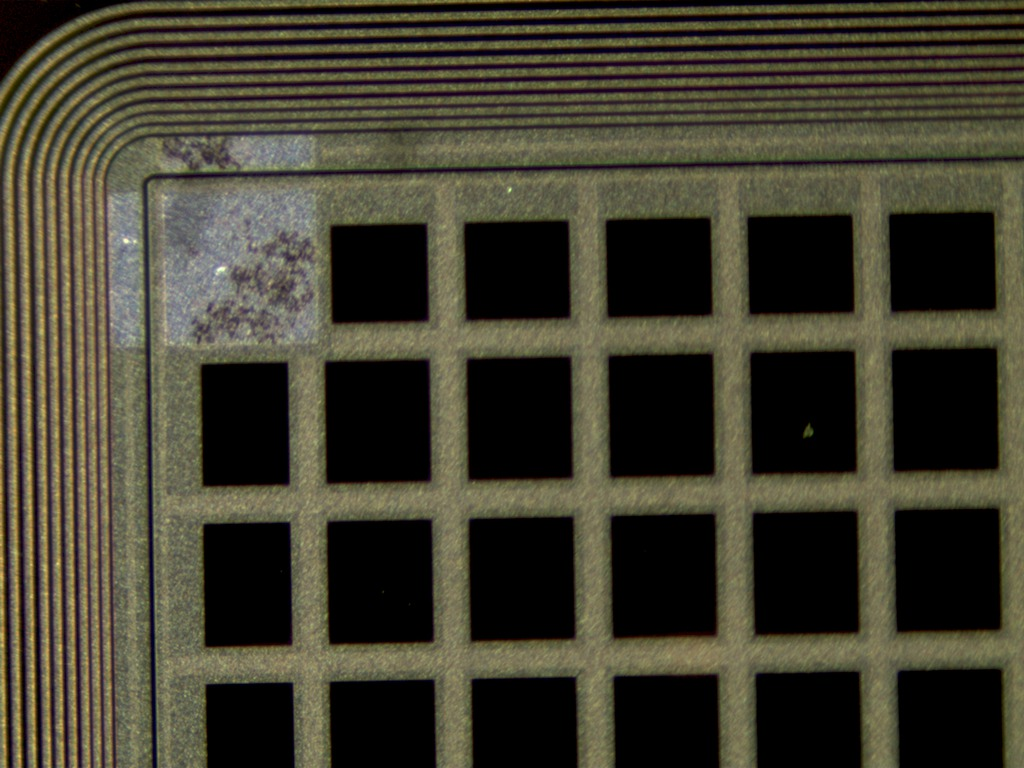
\includegraphics[width=0.7\textwidth]{../images/ch7/vis_insp}
  \caption[Visual inspection of a bare module.]{Visual inspection of a bare module.}\label{fig:vis_insp}
\end{figure}


\subsection{IV-Curve}
\begin{figure}[!h]
  \centering
  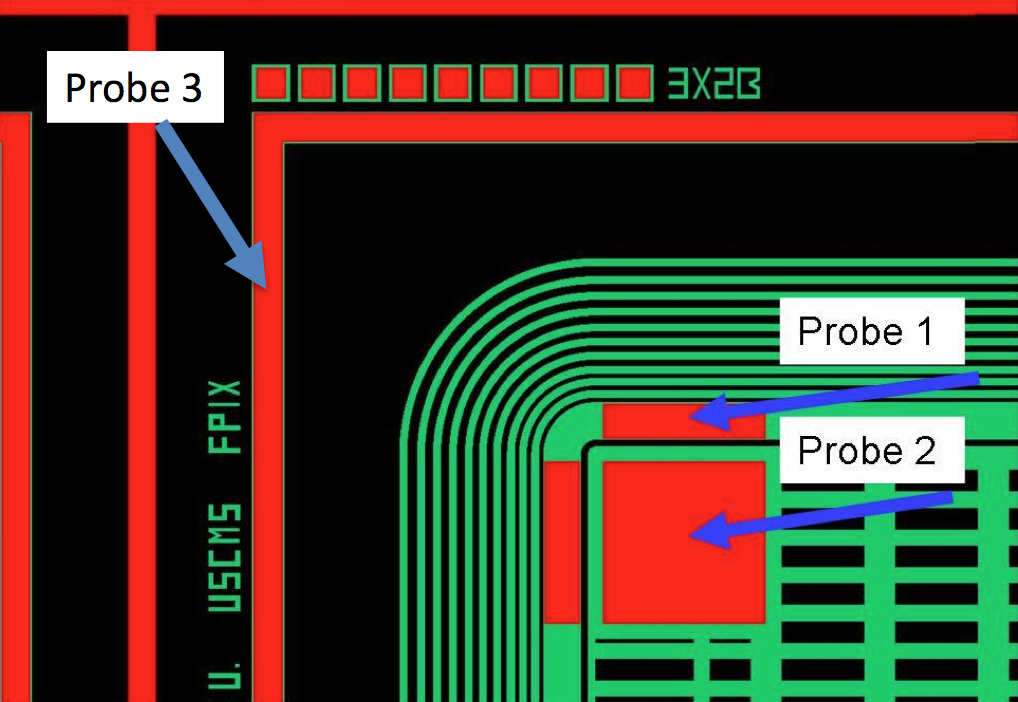
\includegraphics[width=0.7\textwidth]{../images/ch7/sensor_probe_positions}
  \caption[bla for index.]{bla bla.}\label{fig:sensor_probe_positions}
\end{figure}

\begin{figure}[!h]
  \centering
  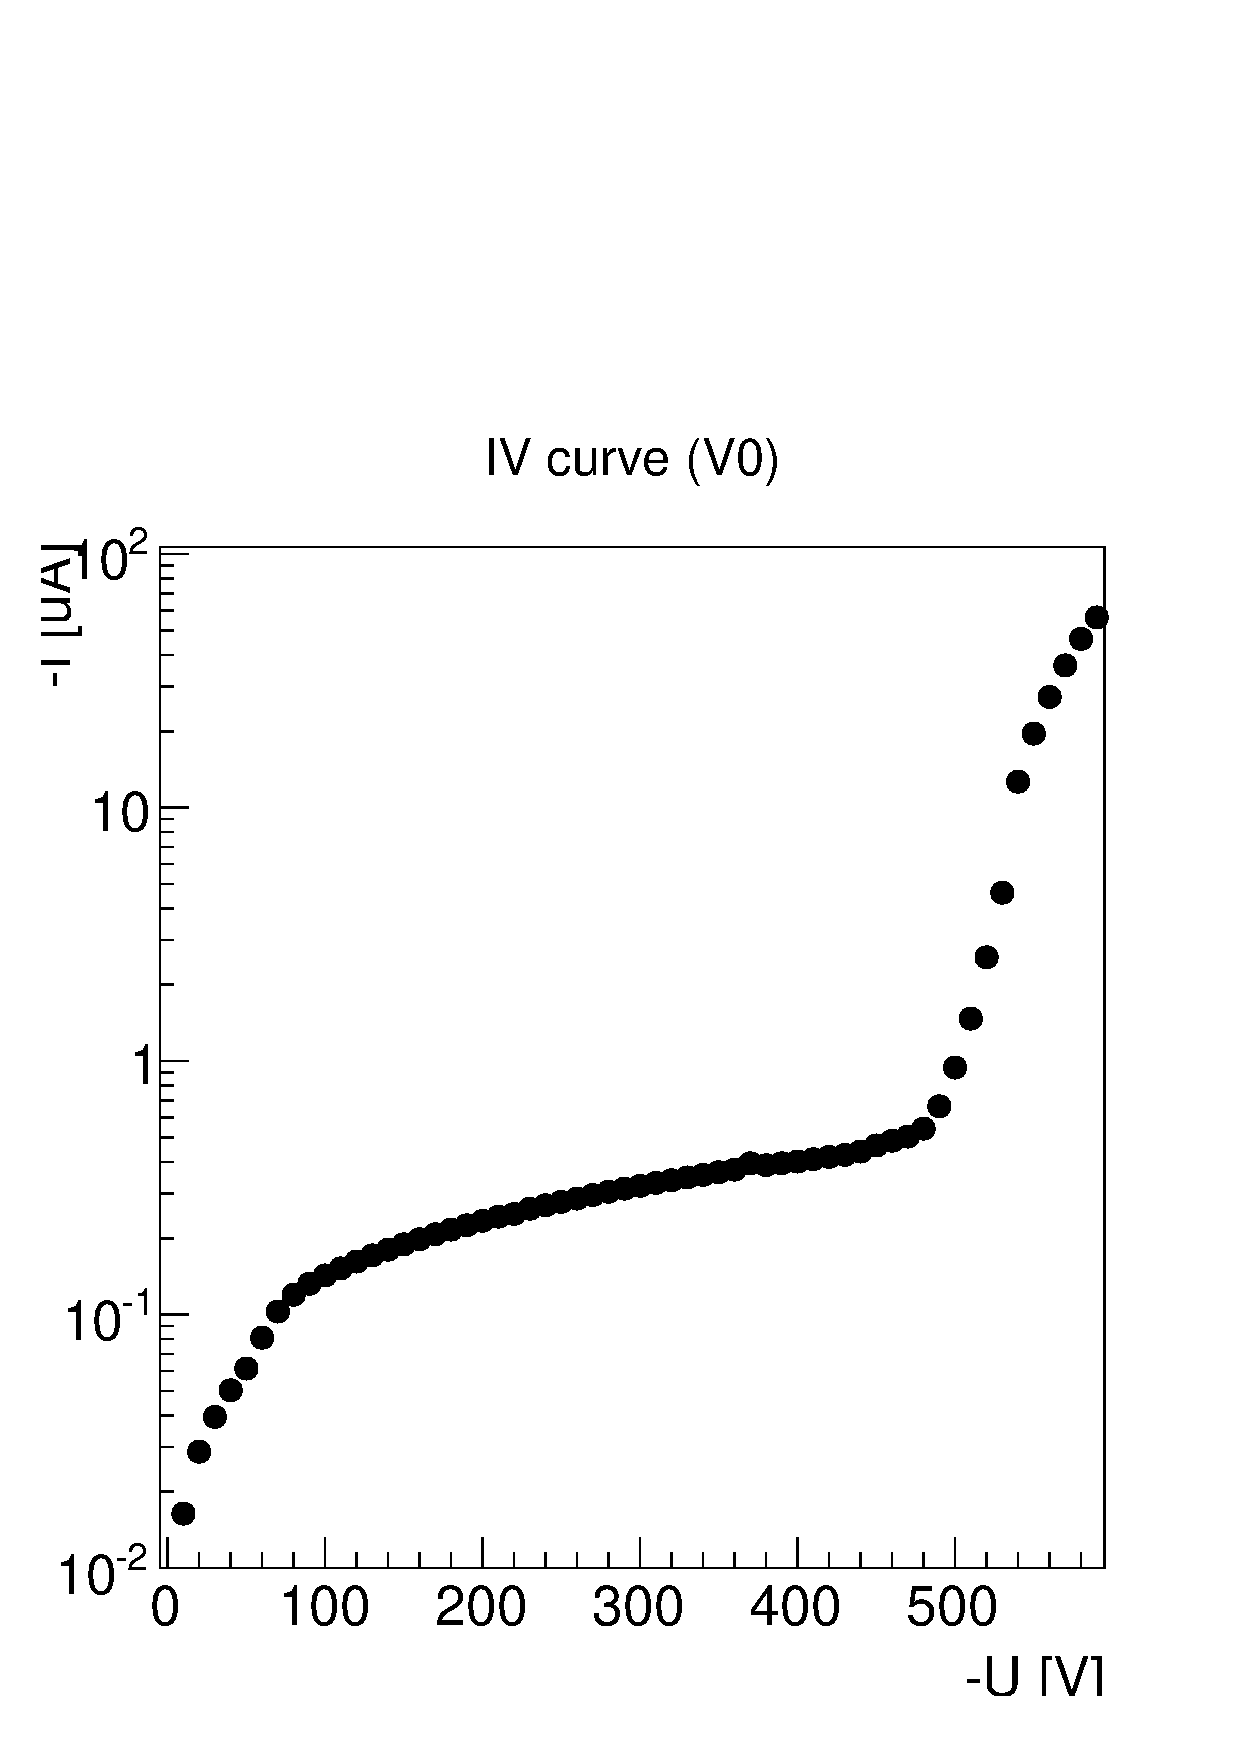
\includegraphics[width=0.7\textwidth]{../images/ch7/iv_test}
  \caption[bla for index.]{bla bla.}\label{fig:vis_insp}
\end{figure}

\subsection{Module assembly}
\begin{figure}[!h]
  \centering
  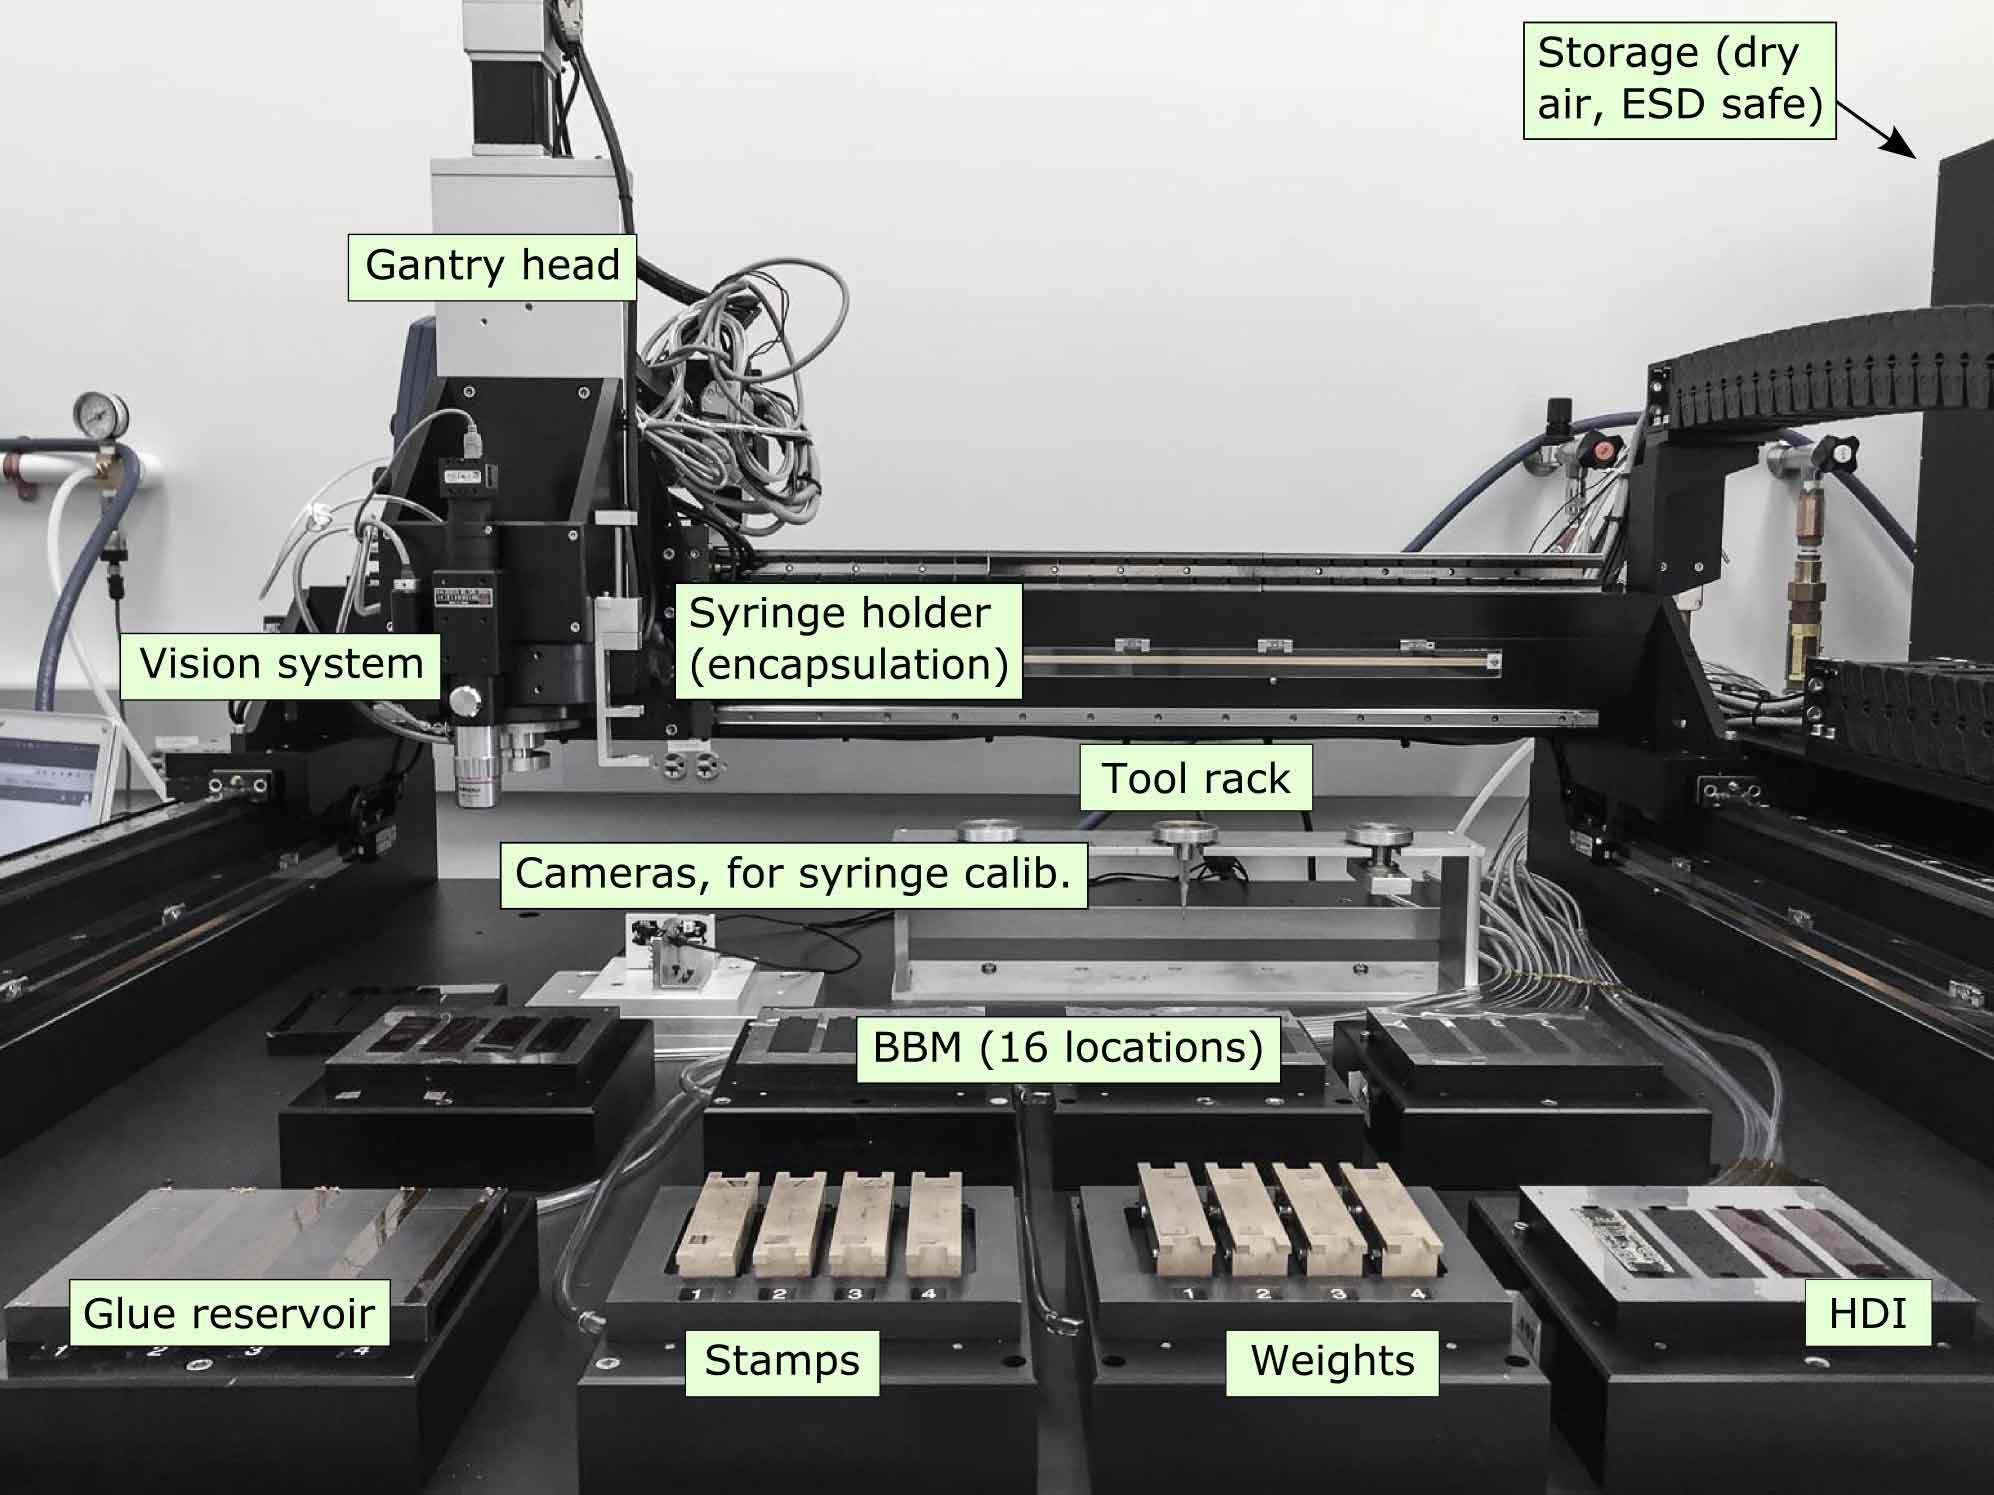
\includegraphics[width=0.7\textwidth]{../images/ch7/gantry}
  \caption[bla for index.]{bla bla.}\label{fig:gantry}
\end{figure}



\subsection{Electrical Test of a Fully assembly Module}
\begin{figure}[!h]
  \centering
  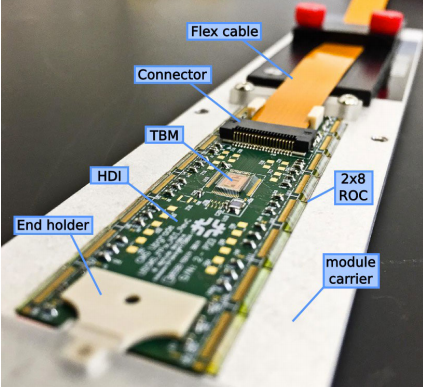
\includegraphics[width=0.7\textwidth]{../images/ch7/fully_asem_mod}
  \caption[bla for index.]{bla bla.}\label{fig:fully_asem_mod}
\end{figure}







\begin{figure}[!h]
  \centering
  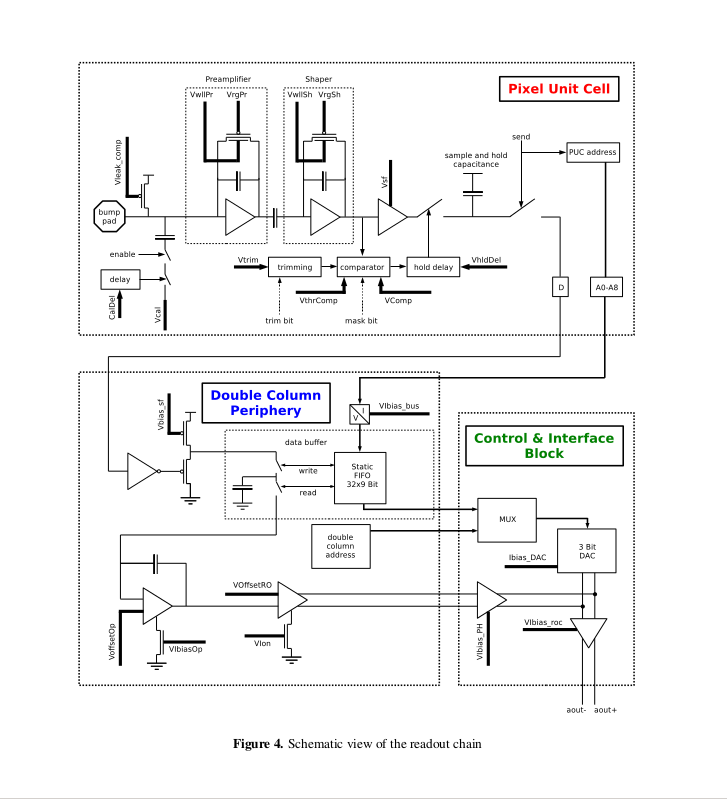
\includegraphics[width=0.7\textwidth]{../images/ch7/pix_unit_cell}
  \caption[bla for index.]{bla bla.}\label{fig:pix_unit_cell}
\end{figure}



\begin{figure}[!h]
  \centering
  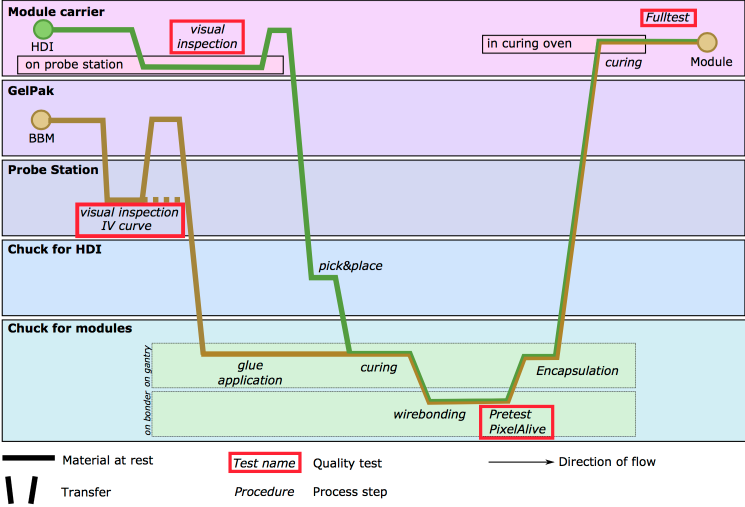
\includegraphics[width=0.7\textwidth]{../images/ch7/unl_workflow2}
  \caption[bla for index.]{bla bla.}\label{fig:unl_workflow2}
\end{figure}

















